\chapter{Intrusion Analysis}

A critical point in improving the robustness of a system and resist to intrusions
is to \ul{know all the intrusions of one or some threat agents} aka attackers;
the reason is that we are sure that our changes improve the robustness and
resilience of a system only if we know all the intrusions.

\begin{center}
   \color{gray}
   \textit{If we know just a \textbf{proper subset} $Sub$ of the possible intrusions $Int$ against a system
   $S$ and if we change $S$ to stop intrusion in $Sub$ only, then this may increase the
   success probability of some intrusions against $S$ in $Int / Sub$}
\end{center}
There is also a formal proof of the above \textit{theorem},
which is a consequence of \textbf{Bayes theorem} and shows the holistic nature of
security,
meaning that you \textbf{cannot} achieve security by \textbf{local} improvements.

The theorem can explain the failure of risk assessment and management solutions
based upon the discovery of a few intrusions against a system (penetration test,
red/purple team, capture the flag) and stresses that automated discovery is needed due to the huge number of intrusions.

\section{Bayes theorem}
\textbf{Bayes Theorem} came out from logistic and operational research and states the following:
\emph{Let us assume there is a group of people that want to go from A to B but all the paths between the two points cross a bridge,
then an increase in the number of bridges may increase the
average time from A to B.}

In \textit{cybersecurity} the increase may be due to lack of information on the \textbf{shortest paths} from A to B.
By increasing the number of paths we increase uncertainty
about the optimal choice at a choke point.
Looking at the theorem from an opposite point of view, a decrease in the number of possible
intrusions ($=paths$) may decrease the time to implement an intrusion.

\section{Measuring \#intrusions}

\subsection{Graph}
Build an oriented graph $OG$ paired with the triple $\langle \textit{system S}, \textit{attacker TA}, \textit{goal G} \rangle$ as following:
\begin{enumerate}
   \item Each node $N$ of $OG$ is paired with a set of access rights of $S = \textit{security status} =SS(N) = $access rights TA has acquired through the previous attacks
   \item Each arc $A$ of $OG$ is labelled with $\langle A, V, M \rangle$ where $A$ is an attack, $V$ a vulnerability
   and $M$ is a module of $S$
   \item The \textit{precondition} of $A$ (i.e. the access rights to execute $A$) are a subset of $SS(N)$
   where $N$ is the source of $A$
\end{enumerate}

\labelitemize{
   \textit{Graph properties}
}{
   \begin{itemize}
      \item $OG$ is acyclic ($TA$ is rational and minimizes its efforts)
      \item No path of $OG$ has multiple occurrences of an arc with the same label
      \item The initial node $I$ is the one where $SS(I)$ is the set of legal access rights of $TA$
      \item A node $FN$ is final if there is at least one path from $I$ to $FN$ and the $FN$ is the first node
      on the path where $SS(FN)$ includes $G$
      \item Any intrusion defines a path from $I$ to a final node
      \item $G$ can be generalized to a set of goals and node $N$ is final if $SS(N)$ belongs to $G$
   \end{itemize}
}

\begin{figure}[htbp]
   \centering
   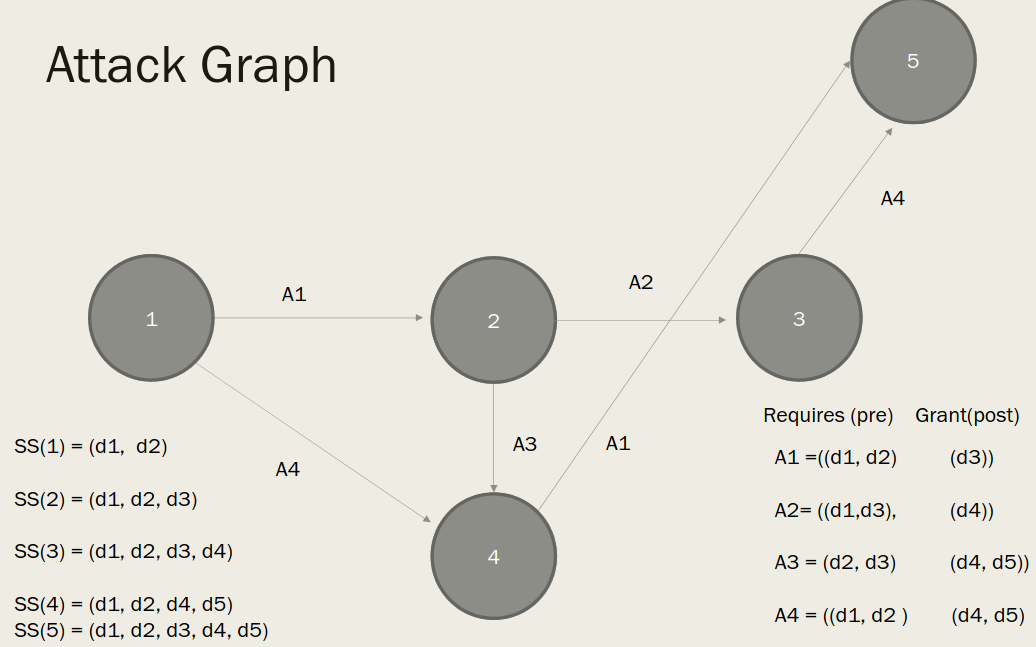
\includegraphics{images/attack_graph.png}
   \caption{Simple attack graph example}
   \label{fig:attack_graph}
\end{figure}
\note{Note that attack graphs assume that attacks \textit{always succeed},
and that access rights are \textit{never lost},
in fact they are always increasing}

Since no defense is considered the acquisition of rights is \textbf{monotonically increasing},
leading to \textbf{huge graphs}, making them computationally unfeasable to be analyzed.
To consider attack failures we need to define an \textbf{attacker state} that also takes into account previous \textbf{failures},
since overall process is not a Markov process because the next action also
depends upon the past history.
However, a detailed modeling of attacks and access rights increases the overall complexity.

\subsection{Tree}

We can simplify the attack graph and represent intrusions with trees:
\begin{enumerate}
   \item A leaf represents an attack enabled by a vulnerability = an elementary attack
   \item a node that is not a leaf represents a complex attack
   \item the subtree rooted in the node shows how a complex attack may be implemented
\end{enumerate}

\begin{itemize}
   \item Each node that cannot be mapped into an elementary attack should be then
   decomposed into a sequence of attack
   \item The leaves of the tree represents the sequence of attacks in an intrusion
   \item We can have an AND/OR trees where a not-leaf node may have AND or OR sons:
   \begin{itemize}
      \item AND = All the attacks that are sons of the node have to be executed
      \item OR = One attack sufficies
      \item The son of AND/OR nodes may be either elementary or complex attacks
   \end{itemize}
   \item Useful to represent or discover a decomposition and possible choices but not to
   discover all intrusions
\end{itemize}

\begin{figure}[htbp]
   \centering
   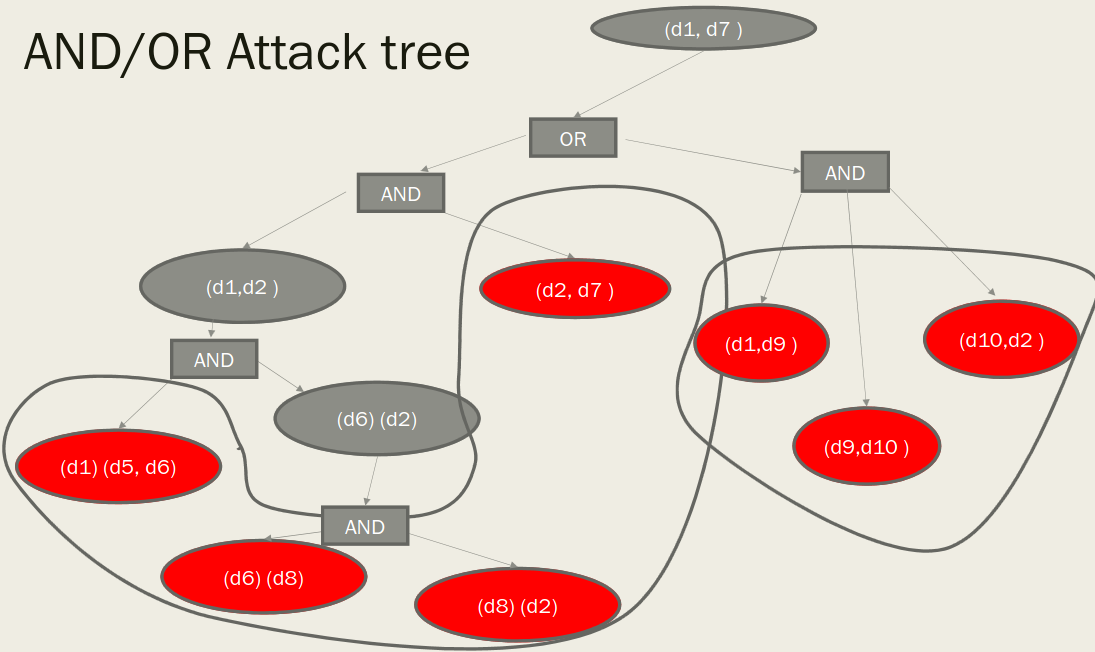
\includegraphics{images/attack_tree.png}
   \caption{Attack tree}
   \label{fig:attack_tree}
\end{figure}

\note{Spoiler alert: intrusion-trees do not work either \smiley}

\subsection{Building and stopping intrusions}
\subsubsection{Building intrusions}
The critical point to discover intrusions is \textbf{adversary emulation},
understanding how
attackers behaves and how they can chain actions to reach a goal.

A starting point may be given by the following properties of an adversary
\begin{enumerate}
   \item Attacks they may execute (due to preferences, tools, resources, know how)
   \item Initial access rights = the legal ones
   \item Initial informations on the system
   \item Final access rights = those in a goal
\end{enumerate}

Recall that an attacker \textbf{cannot} build an attack graph before starting an intrusion
since they have limited
visibility and thus \textit{lack information} on system components.
The attacker interleaves the building of a map of the whole
system with the attacks to reach its goal,
possibly resulting in the execution of \textit{"useless" attacks} that
do not grant any access right to reach the goal,
but are try-and-error steps towards defining such map.

\note{
   Insiders are among the most dangerous attackers because they do not
   have to collect information as they already have a map
}

\subsubsection{Stopping an intrusion}
To stop an attacker we have to stop all its intrusions, 
and to stop an intrusion we need to stop at least one attack in the attack chain in an intrusion (stopping other actions may be more difficult).

It is important to focus only to impactful attacks,
the so-called "useless" ones are negligible in the analysis.
To \textbf{optimize} the security investment,
we should aim to stop attacks useful for several intrusions:
choose the \textit{minimal} number of attacks to stop all intrusions
or
choose a set of attacks to stop such that there is at least \textit{one attack for
each intrusion} and the overall cost is the lowest one.

This optimization problem highlights how to rank vulnerability
to produce a ranking tailored for the target system:
the score of a vulnerability $v$ increases with the number of chains or paths
we can stop by removing the vulnerability $v$.
In the attack graph, 
tailor the score to the pair $\langle system, attacker \rangle$ by considering
the paths the attacker can implement.

\begin{figure}[htbp]
   \centering
   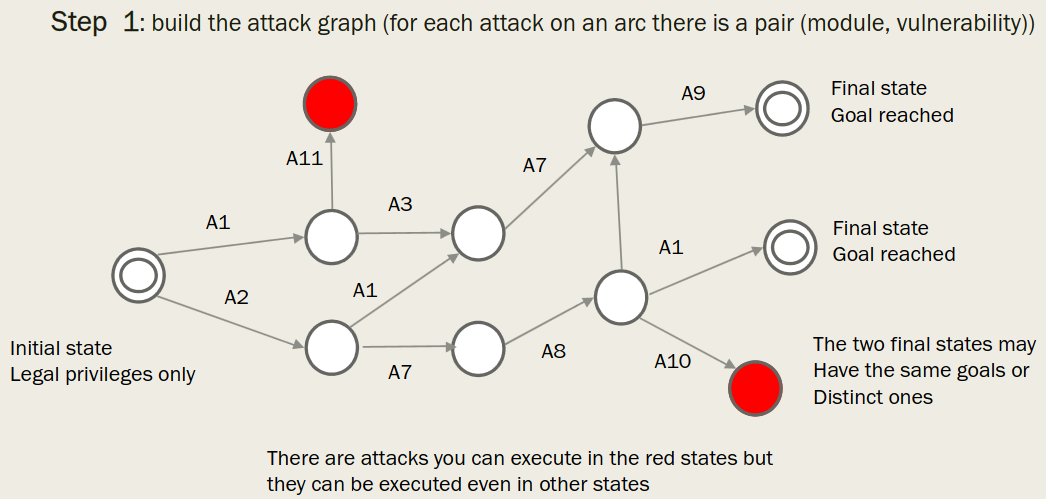
\includegraphics[width=0.48\columnwidth]{images/stop_intrusions_step1.png}
   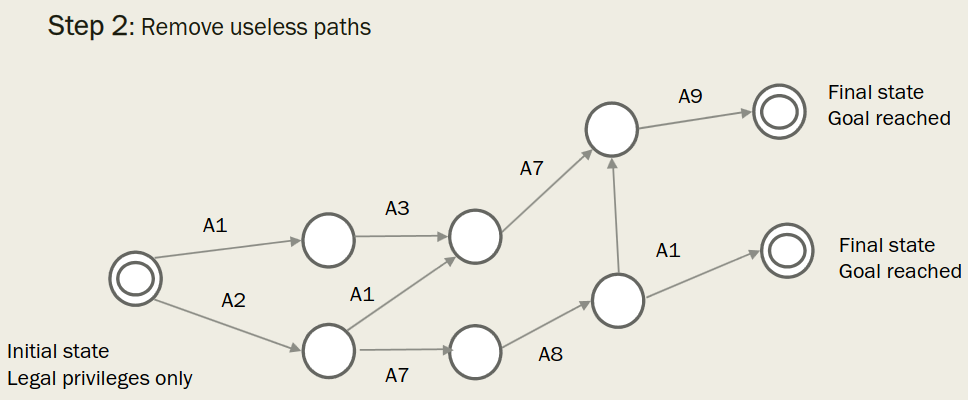
\includegraphics[width=0.48\columnwidth]{images/stop_intrusions_step2.png}\\
   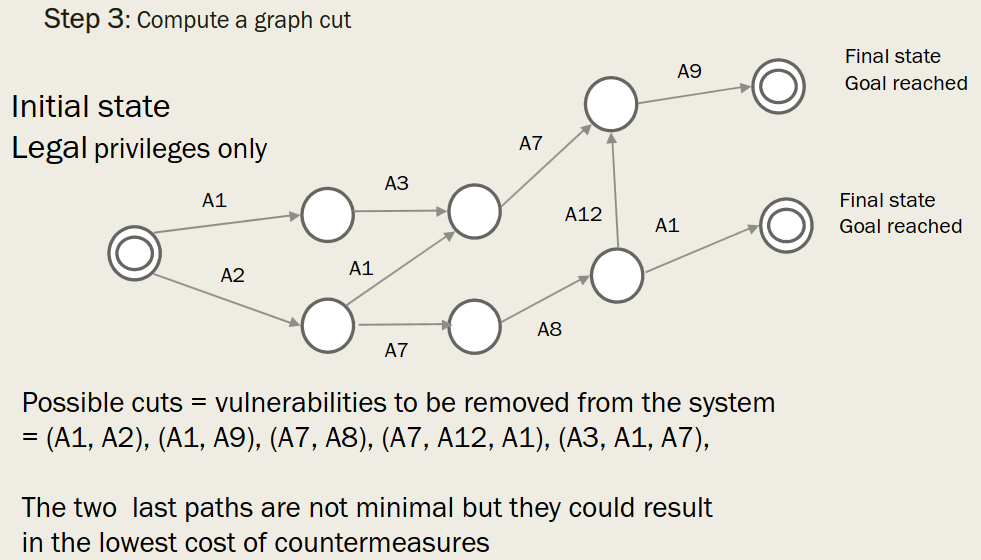
\includegraphics[width=0.48\columnwidth]{images/stop_intrusions_step3.png}
   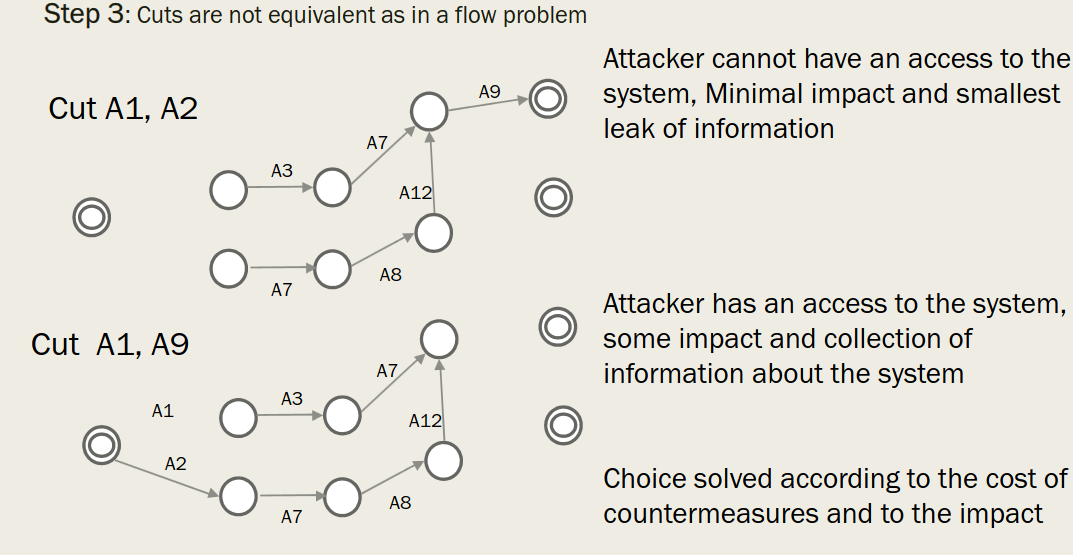
\includegraphics[width=0.48\columnwidth]{images/stop_intrusions_step4.png}
   \caption{Stopping an intrusion using graphs}
   \label{fig:stop_intrusions_steps}
\end{figure}

\section{Automating intrusion}
Even if it's possible to automate attacks, automating intrusions is more complex since
doing so implies having a strategy on ordering attacks and alternating them with actions.\\
In simple cases where the ordering of actions can be easily
discovered automation is possible,
otherwise 
only some phases are automated but not the whole intrusion.
\labelitemize{
   \textit{Intrusion} 
   \textit{steps}
}{
   \begin{itemize}
      \item {\color{gray} Initial access to the system $\longleftarrow$ \textit{Automatable}}
      \item Lateral movement and information collection
      \item {\color{gray} Deployment of malware and encryption $\longleftarrow$ \textit{Automatable}}
   \end{itemize}
}

Instead of using the standard previously described attack graph, a more realistic solution is the following:
\begin{enumerate}
   \item \textbf{Emulate} the behavior of the various attackers
   \item Record each action in a graph
   \item Merge the graphs
   \item Analyze the graph describing their intrusions (\textit{"a-posteriori graph"})
   \item Compute a \textbf{cut} of the graph
\end{enumerate}

An important feature of an \textbf{emulation} is the modeling of attack \textbf{failure} and
how they are handled by an attacker, which can be done in various ways:
\begin{enumerate}
   \item Repeat the attack till it succeeds
   \item Repeat for a predefined number of times and then forget
   \item Choose another action but do not forget the attack and come back later.\\
   The last strategy may result in the discovery of \textbf{black swans},
   which are events with a very low but \textit{\textbf{not} neglectable} probability.
\end{enumerate}

\subsection{Possible attacker's actions}
\subsubsection{Persistence}
An attacker aiming to steal information or to attack later is interested in \textbf{persisting} in a system, i.e. acquiring permanent access to a system.
\note{
   This can be achieved by, for instance, installing a backdoor or some trojan
}
Persistence may be also useful to restart an intrusion from an intermediate point when and if the intrusion has been detected.
The modules the intrusion installs onto the system interact with the \textit{command
and control} infrastructure the attacker has created before starting the
intrusion.
To avoid easy detection and blacklisting,
some attackers store the address of the nodes of the \textbf{C2}\footnote{\textit{Command \& Control}} infrastructure in a public blockchain.

\subsubsection{Evasion}
This class of actions aims to defeat IDS and EDR tools.
Some examples of mechanisms to evade a network signature-based IDS are
\begin{itemize}
   \item Message fragmentation
   \item Message reconstruction
   \item Fake messages
\end{itemize}

Other examples, assessing different defendants countermeasures, are
\textit{token manipulation}, to evade control on authentication, or 
\textit{locally building} container images on a host, evading controls on container images that are first retrieved and then installed on a host.

A frequent choice is to run malicious code inside a VM 
instance, allowing attackers to hide artifacts from security tools that are unable to
monitor activity inside the virtual instance.

\note{
   Notice that the evasion techniques the attacker applies changes the success
   probabilities of some attacks
}

\subsection{Mitre att\&ck matrix}

\texttt{Mitre att\&ck matrix} is {---}a public knowledge database{---} the de facto standard to describe possible behaviors of attackers,
intended as
the \textit{steps} of an intrusion but not the intrusion \textit{itself}.

The matrix format slightly changes according to the type of attack discussed
\labelitemize{
   \textit{Attack types}
}{
   \begin{enumerate}
      \item Pre-Attack
      \item Enterprise
      \item Cloud
      \item ICS
      \item Mobile
   \end{enumerate}
}


Provides a hierarchical definition of behaviours:
\begin{enumerate}
   \item \textbf{Tactics}: \textit{\color{gray}{--}why{--}}\\
   short term goal in an intrusion 
   \item \textbf{Techniques}:  \textit{\color{gray}{--}how{--}}\\
   how the short term goal is reached 
   \item \textbf{Procedure}:  \textit{\color{gray}{--}more detailed how{--}}\\
   detailed implementation of a technique 
\end{enumerate}


\labelitemize{
   \textit{Enterprise Tactics}
}{
\begin{enumerate}
   \item \textbf{Reconnaissance}:
   gathering information to plan future intrusions
   \item \textbf{Resource Development}:
   establishing resources to support operations 
   $\longrightarrow$ \textit{setting up C2 infrastructure}
   \item \textbf{Initial Access}:
   how to get into your network 
   $\longrightarrow$ \textit{spear phishing }
   \item \textbf{Execution}:
   run adversary-controlled code 
   $\longrightarrow$ \textit{running a remote access tool}
   \item \textbf{Persistence}:
   trying to maintain their foothold 
   $\longrightarrow$ \textit{changing configurations}
   \item \textbf{Privilege Escalation}:
   trying to gain higher-level permissions 
   $\longrightarrow$ \textit{leveraging a vulnerability to higher access}
   \item \textbf{Defense Evasion}:
   trying to avoid being detected 
   $\longrightarrow$ \textit{using trusted processes to hide malware}
   
   \item \textbf{Credential Access}: stealing accounts names and passwords 
   $\longrightarrow$ \textit{keylogging}
   \item \textbf{Discovery}: trying to figure out your environment 
   $\longrightarrow$ \textit{exploring what they can control}
   \item \textbf{Lateral Movement}: moving through the environment 
   $\longrightarrow$ \textit{using legitimate credentials to pivot through multiple systems}
   \item \textbf{Collection}: gathering data of interest to the adversary goal 
   $\longrightarrow$ \textit{accessing data in cloud storage}
   \item \textbf{Command and Control}: C2 communication with compromised
   systems 
   $\longrightarrow$ \textit{mimicking normal web traffic to communicate with a victim network}
   \item \textbf{Exfiltration}: stealing data 
   $\longrightarrow$ \textit{transferring data to cloud account}
   \item \textbf{Impact}: manipulate, interrupt, or destroy systems and data 
   $\longrightarrow$ \textit{encrypting data with ransomware}
\end{enumerate}
}

\subsubsection{ICS}
When considering attacks to ICSs,
there are two other tactics that are \textit{not} present in \textit{Enterprise}:
\begin{enumerate}
   \item \textbf{Inhibit Response Function}:
   techniques that adversaries use to hinder the
   safeguards put in place for processes and products.
   They result in the inhibition of
   safety, protection, quality assurance, or operator intervention functions to
   disrupt safeguards that aim to prevent the loss of life, destruction of
   equipment, and disruption of production.
   \item \textbf{Impair Process Control}:
   techniques to disrupt control logic and cause
   malicious effects to processes the target environment controls. 
   Targets may include active procedures or parameters that manipulate the
   physical environment. These techniques can also include prevention or
   manipulation of reporting elements and control logic.
\end{enumerate}

\textit{Exfiltration} is missing because these systems are usually not attacked to steal information,
while some techniques are typical of ICS,
like manipulating an indicator on a host.

\subsubsection{Cloud}
Use of standard malicious software is not taken into account when considering attacks to cloud-based system,
since they are easily detectable.

Instead, a typical way of attacking and exfiltration,
is for attackers to have a cloud account and transfer information from other accounts to theirs,
resulting in stolen information.

% \subsection{Exam Project Ideas}
% Looks for slides of $7^{th}$ \textit{November}.
% Slides $10...14$ provide a list of more specific examples of several tactics.

\section{Caldera}
\textbf{Caldera} is an open-source framework developed by MITRE for the
creation of automated adversary emulation plans.
It is designed to help security teams assess their
organization’s defences by \ul{simulating real-world attacks}
using techniques and tactics mapped to the \texttt{MITRE ATT\&CK} framework.
This automated solution includes a graphical user interface
(\texttt{GUI}) that allows users to easily create and manage custom
attack plans, as well as a range of plugins and modules for
different attack techniques.
It shows an attack in real-time
and allows security teams to identify their weaknesses in a
controlled environment.

The simulation of an \textbf{adversary profile} corresponds to an operation
structured into \textbf{phases}
\begin{itemize}
   \item Each phase involves the execution of an ability,
   so there's a matrix with abilities and phases.
   \item Two abilities in different phases can communicate through facts the
   first one produces. 
   \item A centralized architecture with one server and client-side agents,
   where each agent simulates an attacker on the executing host.
   The server
   administers the operations, plans the actions to be executed and
   returns to the user all the information from by the various agents.
   \item After planning actions to be performed, the server waits for the
   agents to connect and then order them what to do. Each agent
   executes on the host where it runs the action the server chooses.
   \item An agent can be started manually by the user or by another agent
   following some lateral movements in an operation
\end{itemize}


\section{Cascade}
\textbf{Cascade} is a command-and-control (C2) framework developed by MITRE for
use in red team operations and adversary emulation;
it is designed to enable red teams to quickly and
easily create and manage C2 infrastructure, allowing them to
more effectively simulate the actions of a real-world adversary.

Like \textit{Caldera}, \textit{Cascade} is based on the \texttt{MITRE ATT\&CK}
framework, and it is designed to support a wide range of different attack techniques and tactics by being highly modular.
It can be integrated with other tools and platforms to provide a
comprehensive adversary emulation solution for red teams and security practitioners.